\section{System Description}

Our approach to generating visual narratives begins as a linear
process that selects next comic panels based on the contents of previous
panels, choosing randomly among indistinguishably-valid choices.
The concepts we represent formally are {\em transitions}, {\em frames}, and
{\em visual elements}, which we define below.

% XXX how to make this a heading that looks different from a section
% heading?
% \subsection{Visual elements, frames, and transitions}

A {\bf visual element (VE)} is a unique identifier from an infinite set,
each of which is possible to map to a distinct visual representation.
We do not explicitly tag visual elements as specifically characters, props,
or scenery, making the representation agnostic to which of these narrative
interpretations will apply. In the visual rendering of our comics, we
represent VEs as random combinations of shape, color, and size, supplying
additional inputs to the human cognitive processes that may interpret these
elements' narrative role.

A {\bf frame} is a panel template; at the abstract generation level, it
includes an identifier or set of tags and a minimum number of required
visual elements. The reason a frame specifies a {\em minimum} number of VEs
is to allow for augmentation of the frame with pre-existing elements: for
example, the {\em monologue} frame requires at least one visual element,
indicating a single, central focal point, but other visual elements may be
included as bystanding characters or scenery elements.
At the rendering level, a frame includes instructions for where in the
panel to place supplied visual elements.
A {\bf panel} is a frame instantiated by specific visual elements.

% Modifier: visual details overlaid on frames and VEs to add semantic
% coherence to the comic, such as floating emotes, facial expressions, motion
% lines, word balloons, and other text.

Finally, a {\bf transition} is a specification for how a panel should be
formed as the next panel in a sequence, which we describe formally below.

Transition types were first described by
McCloud~\cite{mcCloud1993understanding} % XXX as a means of analyzing
comics. He gave an account of transitions including {\em moment-to-moment},
{\em subject-to-subject}, and {\em aspect-to-aspect}, referring to changes
in temporal state, focal subjects, and spatial point-of-view. As Cohn (XXX
cite ch 4 of visual lang of comics) points out, these transition types are
highly contextual; they presume the reader has a semantic model of the
``story world'' in which the comic takes place. For the sake of
computational generation, we derive a more {\em syntactic} notion of
transition defined purely in terms of frames and (abstract) visual
elements. So, for example, while McCloud could refer to an action-to-action
transition as one where a character is depicted carrying out two distinct
actions, we have no notion of {\em character} and {\em action}, so instead
must refer to which visual elements appear and in which frame. The
rendering of a frame itself may position VEs in such a way that a reader
would read certain actions or meaning into it; however, this kind of reader
interpretation is not modeled to inform generation.

\subsection{Formal Transition Types}

We introduce six formal transition types: {\bf moment}, {\bf add}, {\bf
subtract}, {\bf meanwhile}, and {\bf rendez-vous}, each of which specifies
how a next panel should be constructed given the prior sequence.

\begin{itemize}
\item {\bf Moment} transitions retain the same set of VEs as the previous panel, 
changing only the frame.

\item {\bf Add} transitions introduce a VE that didn't appear in the
previous panel, but might have appeared earlier (or might be completely
new). A new frame may be selected.

\item {\bf Subtract} transitions remove a VE from the previous panel and
potentially choose a new frame.

\item {\bf Meanwhile} transitions select a new frame and show {\em only}
VEs that did not appear in the previous panel, potentially generating new
VEs.

\item {\bf Rendez-vous} transitions select a random subset of
previously-appearing VEs (from anywhere in the sequence) and selects a new
frame to accommodate them.
\end{itemize}

\subsection{Implementation}

Inputs: length constraint, number of starting visual elements
Output: sequence of panels stitched together with transition names

Algorithm:
\begin{itemize}
\item Generate transition sequence based on length constraints
\item Feed transition sequence and starting VEs to panel selector
\item Select next frame and VE set for each new panel based on each
transition
\end{itemize}

Web front-end:
\url{http://www.cs.cmu.edu/~cmartens/comicgen}

XXX Standard ML, JS of Ocaml, JavaScript

Interface:
\begin{figure}[h]
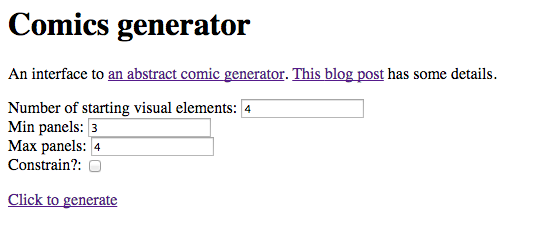
\includegraphics[width=0.5\textwidth]{comicgen-interface.png}
\end{figure}


\section{Generator Output}

(XXX)

\subsection{Example}

\begin{figure}
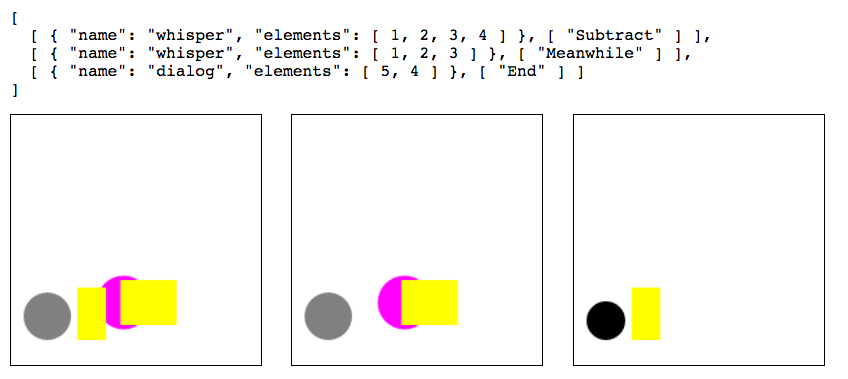
\includegraphics[width=0.5\textwidth]{comicgen-output-1.png}
\end{figure}

\subsection{Constraining generation with Cohn grammars}

Instead of transition types, Cohn's grammar of comics consists of {\em
roles} that each panel plays in the narrative. These roles are {\bf
establisher}, {\bf initial}, {\bf prolongation}, {\bf peak}, and {\bf}
release --- similar to the dramatic arc of standard Western narrative
theories. Formally, Cohn gives the following grammar for sequences of panel
roles:

(XXX paste this in)

Cohn grammars give a holistic structure to the desired output of a comic,
but, like McCloud transitions, they do not inform at a syntactic level how
each panel might be constructed. Our approach is to use Cohn grammars to
guide the selection of syntactically-defined transitions, and, in turn,
realize Cohn's semantic panel roles in terms of the panel's syntactic
relationship to prior panels.

In particular, we enumerate every possible role bigram in Cohn's grammar,
such as {\em initial to prolongation}, {\em prolongation to peak}, and so
on, and describe sets of transition types that could plausibly model the
relationship.

(XXX explain below code)

\begin{Verbatim}[fontsize=\small]
let valid_transitions roles =
      match roles with
        (Establisher, Initial) -> [Moment; Subtract; Add; RendezVous]
      | (Establisher, Prolongation) -> [Moment; Subtract; Add]
      | (Establisher, Peak) -> [Add; Meanwhile]
      | (Initial, Prolongation) -> [Moment; Subtract; Add]
      | (Prolongation, Prolongation) -> [Moment; Subtract; Add]
      | (Prolongation, Peak) -> [Subtract; Add; RendezVous]
      | (Initial, Peak) -> [Subtract; Add; Meanwhile; RendezVous]
      | (Peak, Release) -> [Subtract; Add; RendezVous]
      | _ -> [End] (* error! *)
\end{Verbatim}

\subsection{Example of constrained output}




